\documentclass[../../../../main.tex]{subfiles}

\begin{document}

\section*{第1問}

{\bf [解]}
\begin{align*}
a_1&=1，\quad S_n\xrightarrow{n\to\infty}1\quad\cdots①\\
n(n-2)a_{n+1}&=S_n\quad\cdots②
\end{align*}

②から，
\begin{align*}
n(n-2)(S_{n+1}-S_n)&=S_n\\
n(n-2)S_{n+1}&=(n-1)^2S_n\quad\cdots③
\end{align*}

一方，①から$a_1=1$，②で$n=2$として$a_2=-1\quad\cdots④$である．$n\ge3$の時③から，
\begin{align*}
\frac n{n-1}S_{n+1}=\frac{n-1}{n-2}S_n=\cdots=\frac{3-1}{3-2}a_3
\end{align*}
\begin{align*}
\therefore\ S_n=\frac{n-2}{n-1}\cdot2a_3\quad(n\ge3)
\end{align*}

①から，$S_n=\dfrac{1-2/n}{1-1/n}\cdot2a_3\longrightarrow2a_3=1\quad\therefore\ a_3=\dfrac12$であるから，
\begin{align*}
S_n=\frac{n-2}{n-1}
\end{align*}

これは$n=2$でも成立（$\because④$）する．②から，$n\ge4$の時，
\begin{align*}
a_n=\frac1{(n-1)(n-3)}\cdot\frac{n-3}{n-2}=\frac1{(n-1)(n-2)}
\end{align*}

これは$n=3$で成立．以上から
\begin{align*}
a_n=\begin{cases}1&(n=1)\\-1&(n=2)\\\dfrac1{(n-1)(n-2)}&(n\ge3)\end{cases}
\end{align*}

\newpage

\section*{第2問}

{\bf [解1]}
対称性から，$A(1,0)$，$B(\cos\alpha,\sin\alpha)$，$C(\cos\beta,\sin\beta)$（$0<\alpha\le\pi$，$\alpha<\beta<2\pi$）としてよい．
\begin{align*}
\overline{AB}^2&=(\cos\alpha-1)^2+\sin^2\alpha=2(1-\cos\alpha)=4\sin^2\frac\alpha2\\
\overline{BC}^2&=(\cos\beta-\cos\alpha)^2+(\sin\beta-\sin\alpha)^2=2\{1-(\cos\alpha\cos\beta+\sin\alpha\sin\beta)\}=2(1-\cos(\beta-\alpha))\\
\overline{CA}^2&=2(1-\cos\beta)=4\sin^2\frac\beta2
\end{align*}
である．$P=\overline{AB}^2+\overline{BC}^2+\overline{CA}^2$とおく．

(1)
\begin{align*}
P>8&\iff\cos\alpha+\cos\beta+\cos(\beta-\alpha)<-1\\
&\iff2\cos\frac\alpha2\cos\left(\beta-\frac\alpha2\right)<-2\cos^2\frac\alpha2\quad\cdots①
\end{align*}
である．$\alpha=\pi$の時①は$0<0$となって不適だから，$0<\alpha<\pi$である．この時$\cos\dfrac\alpha2>0$だから，
\begin{align*}
①&\iff\cos\left(\beta-\frac\alpha2\right)<\cos\left(\pi-\frac\alpha2\right)\\
&\iff\left(\pi-\frac\alpha2\right)+2n\pi<\beta-\frac\alpha2<\left(\pi+\frac\alpha2\right)+2n\pi\quad(n\in\mathbb Z)\\
&\iff\pi+2n\pi<\beta<(\pi+\alpha)+2n\pi
\end{align*}

$0<\beta<2\pi$から，$n=0$で
\begin{align*}
①\iff\pi<\beta<\pi+\alpha\iff\triangle ABC\text{は鋭角三角形}
\end{align*}

よって，示された．

\begin{figure}[htb]
\centering
\begin{tikzpicture}[scale=1.8, >=stealth]
  \coordinate (O) at (0,0);
  \draw (O) circle (1);
  \coordinate (A) at (1,0);
  \coordinate (B) at (137:1);
  \coordinate (C) at (280:1);
  \draw (A) -- (B) -- (C) -- (A);
  \draw[gray, dashed] (O) -- (A);
  \draw[gray, dashed] (O) -- (B);
  \fill (O) circle (0.4pt) node[below left] {\scriptsize $O$};
  \fill (A) circle (0.5pt) node[right] {$A$};
  \fill (B) circle (0.5pt) node[above left] {$B$};
  \fill (C) circle (0.5pt) node[below] {$C$};
  \draw pic["\scriptsize $\alpha$", draw, angle radius=8mm] {angle=A--O--B};
\end{tikzpicture}
\caption{単位円に内接する$\triangle ABC$}
\end{figure}

(2)
\begin{align*}
P\le9\iff-\frac32\le\cos\alpha+\cos\beta+\cos(\beta-\alpha)\quad\cdots②
\end{align*}
である．この右辺を$f(\beta)$とおく．$t=\cos\dfrac\alpha2$とすると，$0<t<1$で，
\begin{align*}
f(\beta)=2t\cos\left(\beta-\frac\alpha2\right)+2t^2-1\quad\cdots③
\end{align*}
であり，これは$\cos(\beta-\alpha/2)$の単調増加関数で，$\beta=\pi+\dfrac\alpha2$（$\alpha<\beta<2\pi$を満たす）で最小値
\begin{align*}
f(\beta)=2t^2-2t-1
\end{align*}
をとる．次に$t$で平方完成して
\begin{align*}
f(\beta)=2\left(t-\frac12\right)^2-\frac32
\end{align*}
だから②は示された．等号成立は$t=\dfrac12$かつ$\beta=\pi+\dfrac\alpha2$の時で，$0<\alpha<\pi$だから$\alpha=\dfrac23\pi$，$\beta=\dfrac43\pi$

つまり$\triangle ABC$は正三角形である．

\bigskip
\noindent{\bf [解2]}
右のおりがく．$\triangle ABC$の外接円の半径は$1$だから，正弦定理から，
\begin{align*}
\overline{AB}=2\sin C,\quad\overline{BC}=2\sin A,\quad\overline{CA}=2\sin B
\end{align*}
たから$P=4(\sin^2A+\sin^2B+\sin^2C)$である．

\begin{figure}[htb]
\centering
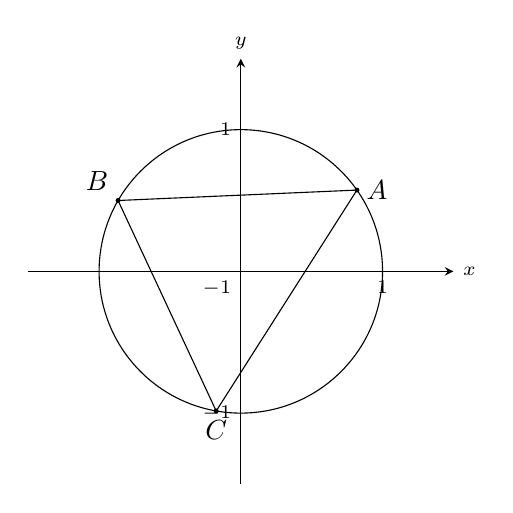
\begin{tikzpicture}[scale=1.8, >=stealth]
  \draw[->] (-1.5,0) -- (1.5,0) node[right] {\scriptsize $x$};
  \draw[->] (0,-1.5) -- (0,1.5) node[above] {\scriptsize $y$};
  \draw (0,0) circle (1);
  \coordinate (A) at (35:1);
  \coordinate (B) at (150:1);
  \coordinate (C) at (260:1);
  \draw (A) -- (B) -- (C) -- (A);
  \fill (A) circle (0.5pt) node[right] {$A$};
  \fill (B) circle (0.5pt) node[above left] {$B$};
  \fill (C) circle (0.5pt) node[below] {$C$};
  \node[below left] {\scriptsize $-1$};
  \node[below] at (1,0) {\scriptsize $1$};
  \node[left] at (0,1) {\scriptsize $1$};
  \node[left] at (0,-1) {\scriptsize $-1$};
\end{tikzpicture}
\caption{正弦定理による別解}
\end{figure}

(1)
\begin{align*}
\frac12P&=\sin^2A+\sin^2B+\sin^2(\pi-A-B)\\
&=\frac{1-\cos2A}2+\frac{1-\cos2B}2+\frac{1-\cos2(A+B)}2
\end{align*}
\begin{align*}
\frac12P&=3-\{\cos2A+\cos2B+\cos2(A+B)\}\\
&=3-\{2\cos(A+B)\cos(A-B)+2\cos^2(A+B)-1\}\\
&=4-2\cos(A+B)\{\cos(A-B)+\cos(A+B)\}\\
&=4-4\cos(A+B)\cos A\cos B
\end{align*}

だから，
\begin{align*}
P>8\iff\cos(A+B)\cos A\cos B<0\iff\cos A\cos B\cos C>0
\end{align*}
（$\because\cos(A+B)=\cos(\pi-C)=-\cos C$）である．$\cos A,\cos B,\cos C$のうち2つが負であるとすると，例えば$B,C$が鈍角となって$B+C>\pi$となり，$0<A$，$A+B+C=\pi$に反するので，$\cos A,\cos B,\cos C>0$となり$\triangle ABC$は鋭角三角形．

(2)
\begin{align*}
\frac12P&=3-\{\cos2A+\cos2B+\cos2C\}\\
&=3-\{2t^2-1+2\cos(A+B)\cos(A-B)\}\quad(t=\cos C)\\
&=4-\{2t^2-2\cos(A-B)\cdot t\}\quad(\because A+B+C=\pi\text{より}\cos(A+B)=-t)\\
&=4+\frac12\cos^2(A-B)-2\left\{t-\frac12\cos(A-B)\right\}^2
\end{align*}

だから，
\begin{align*}
P=8+\cos^2(A-B)-4\left\{t-\frac12\cos(A-B)\right\}^2\le9
\end{align*}

等号成立は$\cos(A-B)=\pm1$かつ$t=\dfrac12\cos(A-B)$の時で，$-\pi<A-B<\pi$だから
\begin{align*}
\cos(A-B)=1,\quad t=\frac12\quad\therefore\ A=B=C=\frac\pi3
\end{align*}

\newpage

\section*{第3問}

{\bf [解]}
2つの整数解を$\alpha,\beta$，2つの虚数解を$z,\bar z$とおく．明らかに$\alpha\beta z\bar z\ne0$．
\begin{align*}
a&=-(\alpha+\beta+z+\bar z)\quad\cdots①\\
1&=\alpha\beta z\bar z=\alpha\beta|z|^2\quad\cdots②\\
c&=-\alpha\beta z\bar z\left(\frac1\alpha+\frac1\beta+\frac1z+\frac1{\bar z}\right)\\
&=-\left(\frac1\alpha+\frac1\beta+\frac{z+\bar z}{|z|^2}\right)\quad(\because②)\quad\cdots③\\
b&=\alpha\beta+(\alpha+\beta)(z+\bar z)+|z|^2\quad\cdots④
\end{align*}

①から，$z+\bar z=2\mathrm{Re}(z)\in\mathbb Z$とかける（$\because\alpha,\beta\in\mathbb Z$）．$z+\bar z=t$（$t\in\mathbb Z$）とおく．④から同様に$|z|^2\in\mathbb Z$が従う．したがって②から，
\begin{align*}
|z|^2=1,\ \alpha\beta=1\quad\therefore\ |z|=1,\ (\alpha,\beta)=(1,1),(-1,-1)\quad\cdots⑤
\end{align*}
とわかる．したがって，$z$を見ると，$|z|=1$かつ$\mathrm{Re}(z)=t/2$から$\mathrm{Im}(z)^2=1-t^2/4$であり，$z$は虚数（$\mathrm{Im}(z)\ne0$）だから$|t|<2$，すなわち$t=0,\pm1$である．このとき
\begin{align*}
z=\frac t2\pm i\sqrt{1-\frac{t^2}4}\qquad(t=0:\ z=\pm i,\quad t=1:\ z=\frac{1\pm\sqrt3i}2,\quad t=-1:\ z=\frac{-1\pm\sqrt3i}2)
\end{align*}

\bigskip
$1^\circ$ $(\alpha,\beta)=(1,1)$の時

①④に代入して
\begin{align*}
a=-(2+t),\quad b=2+2t,\quad c=-(2+t)
\end{align*}
となり，
\begin{align*}
f(x)=x^4-(2+t)x^3+2(1+t)x^2-(2+t)x+1=(x-1)^2(x^2-tx+1)
\end{align*}

②から，$t=0,\pm1$のいずれも$x^2-tx+1=0$の判別式$t^2-4<0$を満たし十分で，
\begin{align*}
(a,b,c)=(-2,2,-2),\ (-3,4,-3),\ (-1,0,-1)
\end{align*}

$2^\circ$ $(\alpha,\beta)=(-1,-1)$の時
\begin{align*}
a=-(-2+t)=2-t,\quad b=2-2t,\quad c=-(-2+t)=2-t
\end{align*}

で，$1^\circ$と同様にしていずれも十分で
\begin{align*}
(a,b,c)=(2,2,2),\ (1,0,1),\ (3,4,3)
\end{align*}

以上から，複号同順として
\begin{align*}
(a,b,c)=(\pm2,2,\pm2),\ (\pm1,0,\pm1),\ (\pm3,4,\pm3)．
\end{align*}

\newpage

\section*{第4問}

{\bf [解]}
(1)
\begin{align*}
f'(x)=\frac1{\sqrt{1+x^2}}
\end{align*}

(2) 題意の曲線$C$上の点は$\begin{pmatrix}x\\y\end{pmatrix}=\theta\begin{pmatrix}\cos\theta\\\sin\theta\end{pmatrix}$と表せるから，もとめる長さ$L$として
\begin{align*}
L&=\int_0^\pi\sqrt{\left(\frac{dx}{d\theta}\right)^2+\left(\frac{dy}{d\theta}\right)^2}\,d\theta\\
&=\int_0^\pi\sqrt{(\cos\theta-\theta\sin\theta)^2+(\sin\theta+\theta\cos\theta)^2}\,d\theta\\
&=\int_0^\pi\sqrt{1+\theta^2}\,d\theta\\
&=\frac12\left[\theta\sqrt{1+\theta^2}+\log\left(\theta+\sqrt{1+\theta^2}\right)\right]_0^\pi\\
&=\frac12\left\{\pi\sqrt{1+\pi^2}+\log\left(\pi+\sqrt{1+\pi^2}\right)\right\}
\end{align*}

\newpage

\section*{第5問}

{\bf [解]}
$f(x)=x^3+3ax^2+3bx$とおき，$A:y=f(x)$，$B:y=c$とする．$f'(x)=3x^2+6ax+3b=3(x^2+2ax+b)$である．$A$，$B$が相異なる3交点を持つには，$f(x)=c$が異なる3実解を持つ，つまり$f$が極大・極小を持ちその間に$c$がある必要がある．そのためには$f'(x)=0$が異なる2実解を持つことが必要で，$x^2+2ax+b=0$の判別式を考えて
\begin{align*}
\frac{D}4=a^2-b>0\iff a^2>b
\end{align*}
が必要．このもとで，$f'(x)=0$の2実解を$\alpha,\beta$（$\alpha<\beta$）とおくと，
\begin{align*}
\alpha=-a-\sqrt{a^2-b},\quad\beta=-a+\sqrt{a^2-b}
\end{align*}

\begin{figure}[htb]
\centering
\begin{tikzpicture}[scale=1.3, >=stealth]
  \draw[->] (-3.6,0) -- (3.6,0) node[right] {\scriptsize $x$};
  \draw[->] (0,-2.2) -- (0,2.6) node[above] {\scriptsize $y$};
  \draw[thick, domain=-3.3:3.3, smooth, variable=\x] plot ({\x},{(\x*\x*\x-3*\x)/6});
  \draw[gray] (-3.3,0.4) -- (3.3,0.4) node[right] {\scriptsize $B:y=c$};
  \node[above] at (2.2,1.9) {\scriptsize $A:y=f(x)$};
  \foreach \p/\lab/\posn in {-2.8/{$\frac{3\alpha-\beta}2$}/below, -1.7/{$\alpha$}/below, 0/{$\frac{\alpha+\beta}2$}/below, 1.7/{$\beta$}/below, 2.8/{$\frac{3\beta-\alpha}2$}/below} {
    \draw[gray, dashed] (\p,-1.6) -- (\p,1.9);
    \node[\posn] at (\p,-1.7) {\scriptsize \lab};
  }
\end{tikzpicture}
\caption{$y=f(x)$と$y=c$のグラフ概形}
\end{figure}

$f$は$x<\alpha$で増加，$\alpha<x<\beta$で減少，$x>\beta$で増加し，$x=\alpha$で極大，$x=\beta$で極小となる．$A,B$が相異なる3交点を持つとき，$c$は極小値と極大値の間にあるから，3交点の$x$座標を$x_1<x_2<x_3$とすると$x_1<\alpha<x_2<\beta<x_3$である．

$d=\sqrt{a^2-b}$とおくと，$\alpha=-a-d$，$\beta=-a+d$である．$u=x+a$とおいて$f$を平行移動すると，
\begin{align*}
f(-a+u)-f(-a)=u^3-3d^2u=:h(u)
\end{align*}
となる（実際，展開して確認できる）．$h$は奇関数で，$h'(u)=3(u^2-d^2)$だから，$h$は$u<-d$で増加，$-d<u<d$で減少，$u>d$で増加し，
\begin{align*}
h(-d)=2d^3,\qquad h(d)=-2d^3,\qquad h(-2d)=-2d^3,\qquad h(2d)=2d^3
\end{align*}
である．$k=c-f(-a)$とおくと，$f(x)=c\iff h(u)=k$（$u=x+a$）であり，異なる3実解を持つことから$-2d^3<k<2d^3$である．

$x_1$に対応する$u_1=x_1+a<-d$は$h(u)=k$の$u<-d$における唯一の解であり，$h$はこの範囲で単調増加で$h(-2d)=-2d^3<k$だから，$u_1>-2d$．同様に，$x_3$に対応する$u_3=x_3+a>d$は$h(u)=k$の$u>d$における唯一の解であり，$h(2d)=2d^3>k$だから，$u_3<2d$．また$u_2=x_2+a\in(-d,d)\subset(-2d,2d)$である．

以上から，$u_1,u_2,u_3\in(-2d,2d)$，すなわち
\begin{align*}
x_1,x_2,x_3\in(-a-2d,-a+2d)=\left(-a-2\sqrt{a^2-b},-a+2\sqrt{a^2-b}\right)
\end{align*}
であり，題意は示された．$\blacksquare$

\newpage

\section*{第6問}

{\bf [解]}
$0<\theta<90\quad\cdots①,\qquad a>0\ (a\in\mathbb R)\quad\cdots②$

(ii)から，$e(\theta)=\cos\theta^\circ+i\sin\theta^\circ$とおくと，
\begin{align*}
z_{n+1}-z_n=e(\theta)(z_n-z_{n-1})
\end{align*}

$z_0=0$，$z_1=a$とあわせて，くり返し用いて，
\begin{align*}
z_{n+1}-z_n=\{e(\theta)\}^na
\end{align*}

$\alpha_n=\dfrac{z_n}{\{e(\theta)\}^n}$とすると，
\begin{align*}
\alpha_{n+1}&=\frac1{e(\theta)}\alpha_n+\frac a{e(\theta)}\\
\alpha_{n+1}-\frac a{e(\theta)-1}&=\frac1{e(\theta)}\left\{\alpha_n-\frac a{e(\theta)-1}\right\}\quad(\because①から e(\theta)\ne1)
\end{align*}

$\alpha_0=0$とから，くり返し用いて，
\begin{align*}
\alpha_n&=\left(\frac1{e(\theta)}\right)^n\left(0-\frac a{e(\theta)-1}\right)+\frac a{e(\theta)-1}\\
z_n&=\frac a{e(\theta)-1}\left\{e(n\theta)-1\right\}
\end{align*}

（$\because$ド・モアブルの定理から$\{e(\theta)\}^n=e(n\theta)$）

これが$z_0=0$に一致する$n$（$n\ge1$）が存在する条件は，$a\ne0$，$e(\theta)-1\ne0$（$\because①②$）だから，
\begin{align*}
&\text{"}e(n\theta)=1\text{なる}n\ge1\text{が存在する"}\\
\iff&n\theta=360m\text{なる}n\in\mathbb N,\ m\in\mathbb Z\text{が存在する}\\
\iff&\theta=\frac mn\cdot360\text{なる}n\in\mathbb N,\ m\in\mathbb Z\text{が存在する}\\
\iff&\theta\text{が有理数}
\end{align*}

よって示された．$\blacksquare$

\newpage

\end{document}
